%----------------------------------------------------------------------
% Problem 2

\begingroup
\allowdisplaybreaks

\newpage
\section*{Problem 2}

\begin{figure}[h]
	\centering
	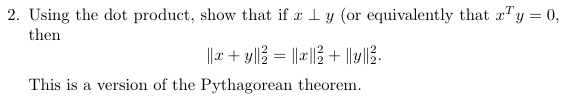
\includegraphics[width=0.8\textwidth]{./images/prob2_statement.png}
\end{figure}

\subsection*{Solution}

Consider the example column vectors $\bv{x},\,\bv{y} \in \R^{n}$ where $n$ is the number of elements in the vector. Then, consider the sum of products given by the expression $\left(\bv{x} + \bv{y}\right)^2$

\begin{align*}
	\left(\bv{x} + \bv{y}\right)^2 &= \left(\bv{x} + \bv{y}\right) \left(\bv{x} + \bv{y}\right) \\
	\\
	&= \bv{x}^T\bv{x} + \bv{x}^T\bv{y} + \bv{y}^T\bv{x} + \bv{y}^T\bv{y}
\end{align*}

Let $\bv{x}$ and $\bv{y}$ be perpendicular such that $\bv{x}^T\bv{y} = \bv{y}^T\bv{x} = 0$. (Recall that dot products are associative) The above expression simplifies such that

\begin{align*}
	\bv{x}^T\bv{x} + \bv{x}^T\bv{y} + \bv{y}^T\bv{x} + \bv{y}^T\bv{y} &= \bv{x}^T\bv{x} + 0 + 0 + \bv{y}^T\bv{y} \\
	\\
	&= \twonorm{\bv{x}} + \twonorm{\bv{y}} 
\end{align*}

Therefore, within the two-norm operation:

\begin{align*}
	\twonorm{\bv{x} + \bv{y}}^2 &= \twonorm{\bv{x} + \bv{y}} \twonorm{\bv{x} + \bv{y}} \\
	\\
	&= \twonorm{\bv{x}^T\bv{x}} + \twonorm{\bv{x}^T\bv{y}} + \twonorm{\bv{y}^T\bv{x}} + \twonorm{\bv{y}^T\bv{y}} \\
	\\
	&= \twonorm{\bv{x}} + \twonorm{\bv{y}} \,\,\,\,\, \textcolor{green}{\checkmark}
\end{align*}